\chapter{التربة الحية}\label{ch:b2:living-soil}

كان آخر كتب تشارلز داروين، وقد نُشر قبل موته بسنة،
عن ديدان الأرض. فقد وضع علامة من الطباشير في حقل قرب
بيته سنة 1842 ونبشها سنة 1871: فوجدها على ثمانية عشر سنتيمترًا
في العمق، وقد دفنتها البُرازات التي رفعتها الديدان إلى السطح
بمعدل قاسه ووزنه وضربه --- عشرة أطنان من
\omterm{def:b2:living-soil:soil}{التربة} في الفدان في السنة تمر عبر أجسادها، حتى إن
«كل الطبقة السطحية من الدُّبال على أي مساحة كهذه قد
مرت، وستمر من جديد، كل بضع سنين عبر أجساد
الديدان». \omterm{def:b2:living-soil:soil}{فالتربة}، بعبارة أخرى، ليست ركيزة تقف عليها
الأحياء بل شيء تصنعه الأحياء. وهذا الفصل
في ذلك الصنع: كيف يصير الصخر \omterm{def:b2:living-soil:soil}{تربة} وكم ببطء، ومن
يعيش فيها وبأي أعداد، وكيف تُفكَّك المادة الميتة وما
يبقى، وكيف تساوم جذور النبات الفطريات والبكتيريا على ما لا
تناله وحدها، وكم بسرعة تُفقد \omterm{def:b2:living-soil:soil}{تربة} استغرق بناؤها عشرة آلاف سنة.

\section{ما التربة}

\begin{definition}[التربة وآفاقها]\label{def:b2:living-soil:soil}
\index{تربة}\index{أفق تربة}\index{دُبال}\index{تجوية}\index{تكوّن التربة}
\emph{التربة} طبقة المادة المعدنية المجوّاة والمادة العضوية
والماء والهواء والكائنات التي تغطي اليابسة وتعيل
النبات: فنحو نصف حجمها مسام، تمتلئ بالماء أو بالهواء
بنسب متغيرة، والنصف الصلب حبيبات معدنية ---
رمل (\qtyrange{0.05}{2}{mm})، وغرين (\qtyrange{2}{50}{\micro m})،
وطين (دون \qty{2}{\micro m})، وتعطي نسبها
\emph{القوام} --- مع بضعة في المئة من المادة العضوية التي
تحكم معظم خصائصها. ويُظهر مقطع التربة
\emph{آفاقًا}: الأفق \emph{O} من الفُتات والمادة العضوية المتحللة
جزئيًا عند السطح؛ والأفق \emph{A} الداكن من التربة
المعدنية الممتزجة \emph{بالدُّبال}، وهو البقية الغروية الداكنة الثابتة
من التحلل؛ والأفق \emph{B} تحته، ويُغسل إليه الطين
والحديد والمادة المنحلة وفيه تتراكم؛
والأفق \emph{C} من الصخر الأم المجوّى؛ ثم صخر القاع. و
تُصنع التربة (وهو \emph{تكوّن التربة}) بخمسة عوامل --- المادة
الأم، والمناخ، والكائنات، والتضاريس، والزمن --- وهي
تُصنع ببطء: فالتجوية تنتج ما رتبته \qty{0.1}{mm} من
التربة في السنة، فيكون المتر من التربة عشرة آلاف سنة من العمل.
\end{definition}

\begin{omfigure}
\begin{tikzpicture}[every node/.style={font=\scriptsize}]
  \fill[brown!25!black!60] (0,5.4) rectangle (4,5.8); \node[right] at (4.2,5.6) {O: فُتات وطحالب ومادة متحللة جزئيًا (بضعة سنتيمترات)};
  \fill[brown!60!black] (0,4.2) rectangle (4,5.4); \node[right, align=left] at (4.2,4.8) {A: تربة معدنية ممتزجة بالدُّبال، داكنة، ذات بنية فُتاتية؛\\ ومعظم الجذور ومعظم الكائنات (\qtyrange{10}{30}{cm})};
  \fill[brown!70!orange!80] (0,2.4) rectangle (4,4.2); \node[right, align=left] at (4.2,3.3) {B: تراكم الطين وأكاسيد الحديد والكربونات\\ المغسولة من فوق؛ وقليل من الجذور (\qtyrange{30}{100}{cm})};
  \fill[gray!50!brown!60] (0,1.0) rectangle (4,2.4); \node[right, align=left] at (4.2,1.7) {C: صخر أم مجوّى، شظايا في حشوة ناعمة};
  \fill[gray!70] (0,0) rectangle (4,1.0); \node[right] at (4.2,0.5) {R: صخر القاع};
  \foreach \x in {0.4,1.3,2.5,3.4} \draw[brown!30!black, thick] (\x,5.4) .. controls (\x+0.2,4.8) and (\x-0.2,4.4) .. (\x+0.1,3.6);
  \foreach \x/\y in {0.7/3.0, 2.0/2.7, 3.2/3.3, 1.5/1.6, 3.0/1.9} \fill[gray!80] (\x,\y) ellipse (0.18 and 0.1);
  \draw[<->, thick] (-0.4,5.8) -- (-0.4,0) node[midway, left, rotate=90, anchor=south] {نحو متر إلى مترين};
\end{tikzpicture}

{\small مقطع \omterm{def:b2:living-soil:soil}{تربة}. المادة العضوية تدخل من الأعلى وتُستهلك
وهي تنزل؛ والمادة المعدنية تُطلق في الأسفل
وترفعها الجذور والحيوانات؛ والمادة المنحلة تسافر
نازلةً مع الماء وتُمسك في الأفق B.}
\end{omfigure}

\begin{proposition}[لماذا يهم الطين والدُّبال]\label{prop:b2:living-soil:cec}
\index{السعة التبادلية للشوارد الموجبة}\index{طين}\index{بنية التربة}\index{سعة حقلية}
تحمل جسيمات الطين والدُّبال شحنات سالبة على سطوحها
وتمسك، بالجذب الكهرساكن، احتياطًا من الشوارد الموجبة
القابلة للتبادل --- $\mathrm{Ca^{2+}}$ و$\mathrm{Mg^{2+}}$ و$\mathrm{K^{+}}$ و$\mathrm{NH_4^{+}}$ --- تسحبها
جذور النبات بمبادلة $\mathrm{H^{+}}$ بها. وهذه
\emph{\omterm{prop:b2:living-soil:cec}{السعة التبادلية للشوارد الموجبة}} مصرف \omterm{def:b2:living-soil:soil}{التربة} الغذائي؛ فالرمل
لا سعة له تقريبًا (بضعة سنتيمولات من الشحنة في الكيلوغرام)، والطميّ
الطيني الغني بالدُّبال أكبر منه بخمسين ضعفًا، وتختلف خصوبة الاثنين
تبعًا لذلك. والسطوح نفسها تمسك الماء: \omterm{def:b2:living-soil:soil}{فالتربة} الرملية
تنضب في غضون يوم إلى \emph{\omterm{prop:b2:living-soil:cec}{سعة حقلية}} قدرها عُشر
حجمها، ويمسك الطميّ ثلثًا، والفرق هو ما يملكه المحصول
بين مطرتين. والدُّبال، مع الهيفات الفطرية ومفرزات
الجذور ومخاط الديدان، يلصق الحبيبات المعدنية في
\emph{تجمعات}، وهي البنية الفتاتية التي تدع مسامها الهواءَ والماءَ
والجذور تمر --- وهي الخاصة التي تميز \omterm{def:b2:living-soil:soil}{التربة} عن
الرسوب والتي تتلفها الحراثة والانضغاط أولًا.
\end{proposition}

\section{من يعيش هناك}

\begin{proposition}[مجتمع التربة]\label{prop:b2:living-soil:community}
\index{شبكة غذاء التربة}\index{آكل الحطام}\index{دودة الأرض}\index{كتلة التربة الحيوية}
الغرام من \omterm{def:b2:living-soil:soil}{التربة} السطحية الخصبة يحمل نحو $10^{9}$ خلية بكتيرية
من نحو عشرة آلاف نوع، ومئة متر من الهيفات الفطرية، و$10^{4}$
أوّليّات، وبضع عشرات من الخيطيات وحفنة من العث
والقافزات الذنبية؛ والمتر المربع يحمل بضع مئات من ديدان الأرض، و
تحت الحيوانات المرئية كتلة حية قدرها عدة أطنان في
الهكتار --- تضاهي ما يستطيع الهكتار نفسه إعالته من الماشية.
والمجتمع \emph{شبكة غذاء حطامية}: فالبكتيريا والفطريات
(أي \emph{المحلِّلات}) تأكل المادة الميتة وتأكلها الأوّليّات
والخيطيات (أي راعيات المجهريات)، وتأكلها العث
والخيطيات المفترسة، وهي تغذي الحريشات والخنافس؛ و\emph{آكلات
الحطام} --- ديدان الأرض وأم أربعة وأربعين وقمل \omterm{def:b2:plant-meristems:wood}{الخشب} والنمل الأبيض
والقافزات الذنبية --- تأكل الفُتات نفسه بما عليه من مجهريات،
فتفتته ألف ضعف وتضاعف السطح الذي
تهاجمه المجهريات. والراعيات تهم بما يفوق أعدادها: فهي بأكلها
البكتيريا تطلق النتروجين المحبوس في الخلايا البكتيرية
أمونيومًا، \omterm{def:b2:living-soil:soil}{والتربة} التي فيها أوّليّات وخيطيات تعدّن
النتروجين أسرع من \omterm{def:b2:living-soil:soil}{التربة} التي فيها بكتيريا وحدها. وديدان الأرض هي
\emph{مهندسات النظام البيئي}: فأنفاقها مسام \omterm{def:b2:living-soil:soil}{التربة}
الكبيرة، وبرازاتها أغنى التجمعات، وديدان
مرج تنقل بضعة أطنان من \omterm{def:b2:living-soil:soil}{التربة} في الهكتار عبر
أمعائها كل سنة، كما قاس داروين.
\end{proposition}

\begin{omfigure}
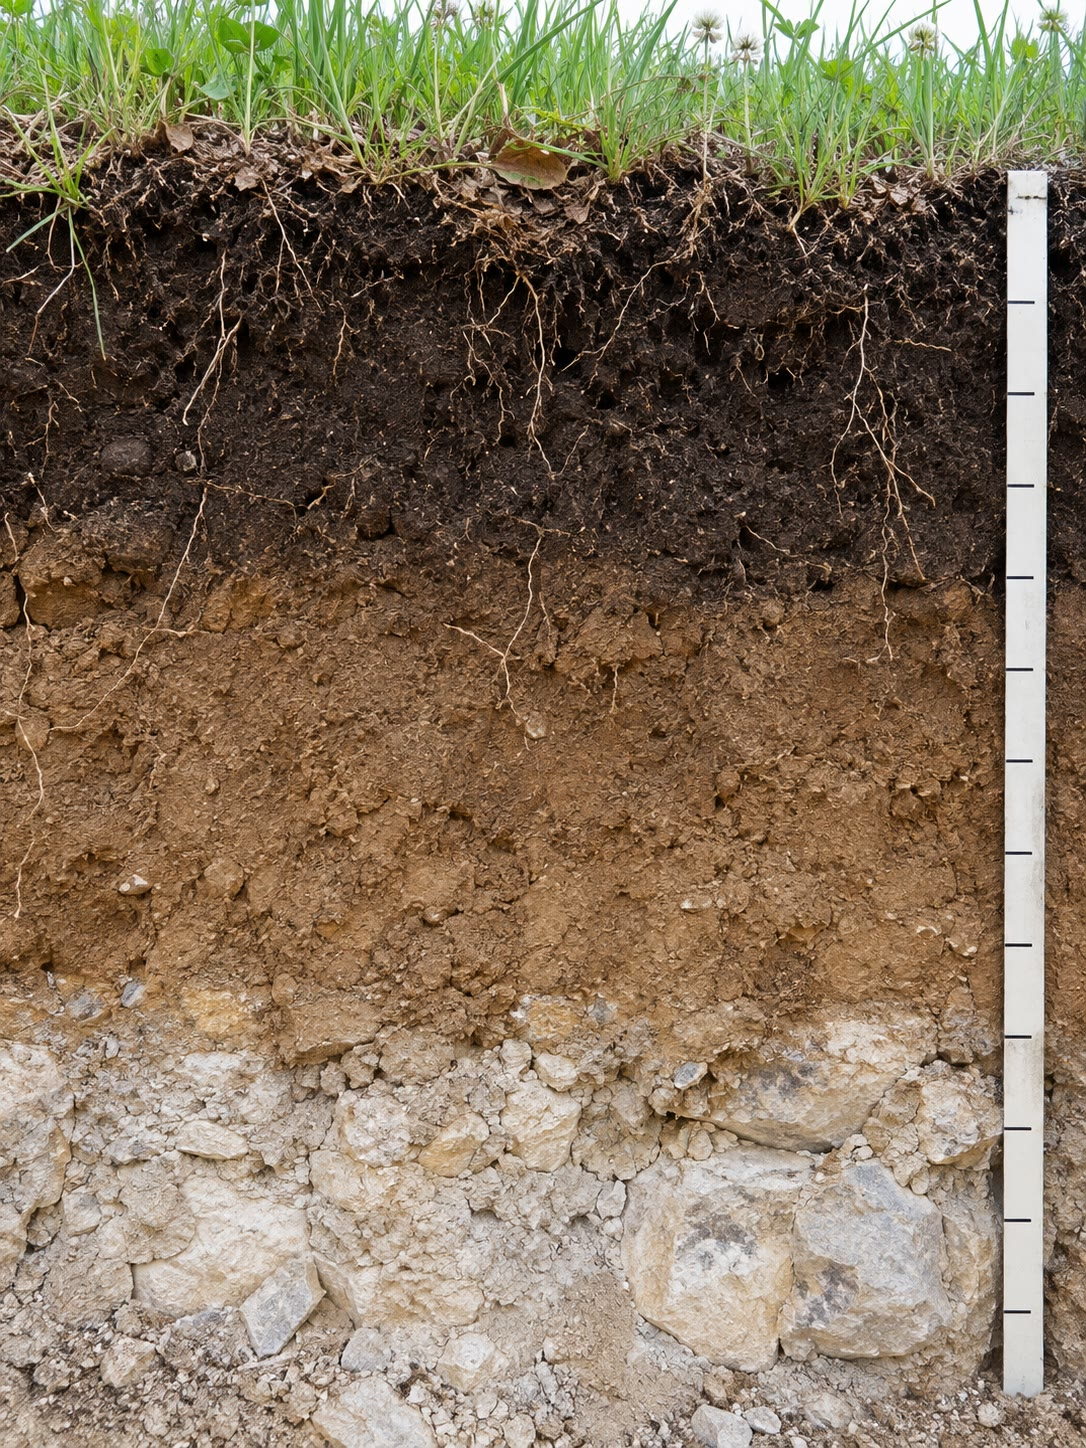
\includegraphics[width=0.21\linewidth]{images/book4/ai/b4-26-soil-profile.jpg}\hspace{0.025\linewidth}
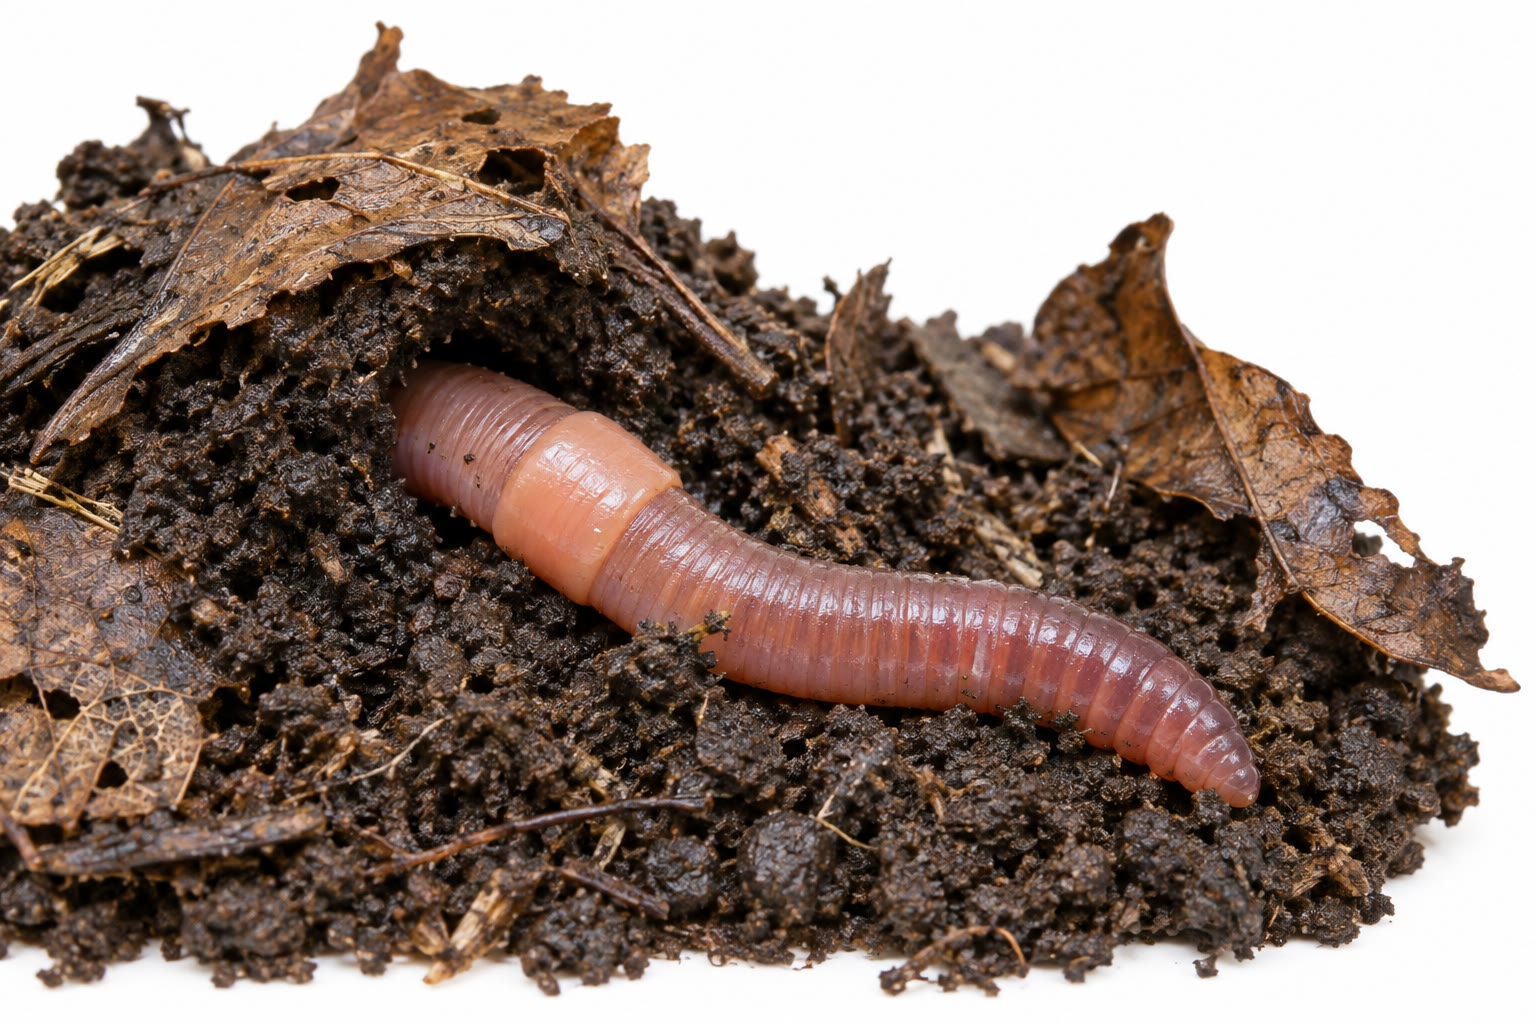
\includegraphics[width=0.42\linewidth]{images/book4/ai/b4-26-earthworm.jpg}\hspace{0.025\linewidth}
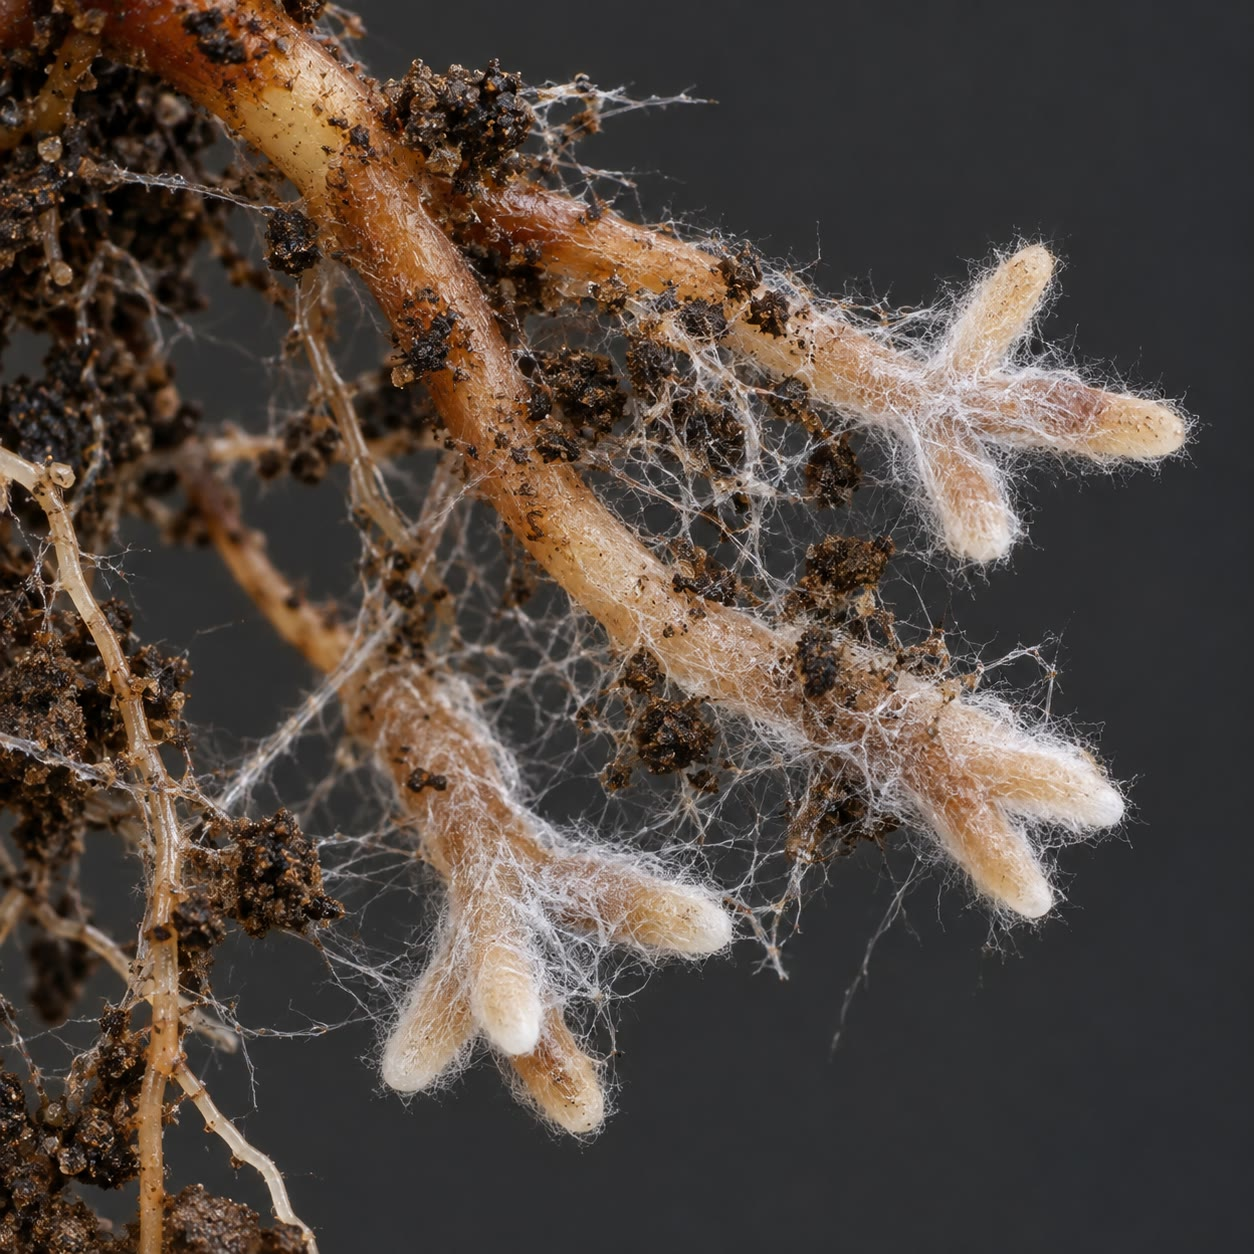
\includegraphics[width=0.28\linewidth]{images/book4/ai/b4-26-mycorrhiza.jpg}

{\small \omterm{def:b2:living-soil:soil}{التربة} واثنان من صانعيها. إلى اليسار: مقطع في ضفة
مقطوعة، \omterm{def:b2:living-soil:soil}{والتربة} السطحية الداكنة تتدرج نازلةً إلى صخر شاحب مجوّى. وفي الوسط:
دودة أرض في نفقها. وإلى اليمين: جذر بغمده
الميكوريزي الخارجي والهيفات التي تمده في \omterm{def:b2:living-soil:soil}{التربة}.}
\end{omfigure}

\section{التحلل}

\begin{theorem}[خبو الفُتات ونسبة الكربون إلى النتروجين]\label{thm:b2:living-soil:decay}
\index{تحلل}\index{خبو الفُتات}\index{نسبة C:N}\index{تمعدن}\index{تثبيط}
يتحلل الفُتات بمعدل يتناسب مع ما يبقى،
$\mathrm{d}L/\mathrm{d}t = -kL$، فيكون $L = L_0 e^{-kt}$ مع
\emph{ثابت خبو} $k$ قدره نحو 1 في السنة للعشب
وأوراق النفضيات في غابة معتدلة، و$0.3$ لإبر الصنوبريات،
وعدة وحدات في السنة في المناطق المدارية الرطبة و$0.05$ في التندرا؛
والدخل الثابت $I$ في السنة يبني طبقة فُتات قدرها $I/k$. والخبو
تتحكم فيه الحرارة والرطوبة و\emph{نوعية} الفُتات:
أي محتواه من النتروجين، ومحتواه من اللغنين، ونسبة
الكربون إلى النتروجين. وللمجهريات $\mathrm{C:N} \approx 8$ وهي
تحتفظ بنحو \qty{40}{\%} من الكربون الذي تأكله، فتحتاج نتروجينًا
واحدًا لكل $8/0.4 = 20$ كربونًا من الغذاء: فالفُتات الذي $\mathrm{C:N}$ فيه
دون 25 نحوًا يطلق الأمونيوم وهو يتحلل
(وهو \emph{التمعدن})، أما الفُتات فوق ذلك --- كالقش عند 80،
\omterm{def:b2:plant-meristems:wood}{والخشب} عند 400 --- فيجعل المجهريات تلتقط النتروجين من \omterm{def:b2:living-soil:soil}{التربة}
(وهو \emph{التثبيط})، فتجوّع النبات حتى يُتنفَّس الكربون
بعيدًا وتهبط النسبة. ولذلك يخفض القش الطازج
المحروث المحصولَ، وتغذيه بقايا البقوليات،
ويحتاج كوم السماد العضوي الاثنين.
\end{theorem}
\begin{proof}
أما النسبة: فالمجهريات التي تأكل فُتاتًا فيه $c$ كربون لكل
نتروجين تستوعب $0.4c$ كربونًا، ولتبني كتلة حيوية عند
$\mathrm{C:N} = 8$ تحتاج $0.4c/8 = c/20$ نتروجينًا؛ والفُتات
يمد 1. فإن كان $c < 20$ فُضل نتروجين يُطلق
أمونيومًا؛ وإن كان $c > 20$ كان هناك عجز يُؤخذ من \omterm{def:b2:living-soil:soil}{التربة}. أما
العتبة 25 في العمل فتعكس كفاءة احتفاظ أدنى قليلًا
من 0.4. وأما طبقة الفُتات: فالمعادلة $\mathrm{d}L/\mathrm{d}t = I - kL$
حالتها المستقرة $I/k$، ويُقترب منها بثابت زمني $1/k$؛ \omterm{def:b2:biogeochemical-cycles:reservoir}{وزمن
مكث} الفُتات $1/k$، وهو سنة في غابة زان
وعشرون في التندرا.
\end{proof}
\begin{proof}[شواهد]
تجارب أكياس الفُتات --- كتل معلومة من الأوراق في أكياس شبكية،
تُدفن وتُوزن على فترات --- أعطت القانون الأسّي
وثوابته عبر كل منطقة حيوية (أولسون، 1963)، وبيّنت بمقاسات شبك
مختلفة أن استبعاد حيوانات \omterm{def:b2:living-soil:soil}{التربة} ينصّف
المعدل: فالمجهريات تقوم بالكيمياء لكن الحيوانات تقرر الوتيرة.
وعبر قارة، تتحلل الورقة نفسها في سنة في جورجيا
وفي ثمان في ألاسكا، بنسبة التبخر النتحي الفعلي،
وهو جداء الدفء والماء.
\end{proof}

\begin{omfigure}
\begin{tikzpicture}
\begin{axis}[
  width=0.72\linewidth, height=5.6cm,
  axis x line=bottom, axis y line=left,
  xmin=0, xmax=6, ymin=0, ymax=105,
  xlabel={السنوات}, ylabel={كتلة الفُتات الباقية (\%)},
  xlabel style={font=\small, at={(axis description cs:0.5,-0.13)}, anchor=north},
  ylabel style={font=\small},
  tick label style={font=\small},
  legend style={font=\scriptsize, at={(0.5,-0.3)}, anchor=north, draw=none, legend columns=2},
  clip=false,
]
\addplot[very thick, omDef, domain=0:6, samples=60] {100*exp(-2*x)};
\addlegendentry{ورقة غابة مدارية، $k = 2$}
\addplot[very thick, omThm, domain=0:6, samples=60] {100*exp(-1*x)};
\addlegendentry{ورقة زان، $k = 1$}
\addplot[very thick, omProp, domain=0:6, samples=60] {100*exp(-0.3*x)};
\addlegendentry{إبرة تنوب، $k = 0.3$}
\addplot[very thick, gray, domain=0:6, samples=60] {100*exp(-0.05*x)};
\addlegendentry{طحلب تندرا، $k = 0.05$}
\end{axis}
\end{tikzpicture}

{\small الخبو الأسّي للفُتات. نصف ورقة الزان يزول
في ثمانية أشهر؛ ونصف \omterm{def:b2:plant-life-cycles:moss}{طحلب} التندرا في أربع عشرة سنة؛ والبقية
التي لا يستطيع مجهري ولا حيوان إنهاءها تصير دُبالًا.}
\end{omfigure}

\begin{proposition}[الدُّبال وحوض كربون التربة]\label{prop:b2:living-soil:humus}
\index{دُبال}\index{كربون التربة العضوي}\index{تنفس التربة}
بضعة في المئة من كربون الفُتات يفلت من الأكسدة التامة
فيصير \emph{دُبالًا}: وهو مزيج داكن لا شكل له من بقايا
مجهرية ولغنين متغير ومركبات نباتية، مرتبط بالطين
والحديد ومقفل في التجمعات، يتحلل بأزمنة مكث من
عقود إلى آلاف السنين. والدُّبال هو حيث تعيش خصوبة \omterm{def:b2:living-soil:soil}{التربة}
--- فمعظم نتروجينها وتبادلها الشاردي، ونصف إمساكها للماء ---
وهو أكبر حوض للكربون العضوي على اليابسة،
\qty{1700}{GtC} في المتر العلوي، أي ضعف ما في الغلاف الجوي. و
ميزانه الدخل ناقص الخبو، $\mathrm{d}H/\mathrm{d}t = I_h - k_hH$:
فعند $k_h \approx 0.02$ في السنة تحمل \omterm{def:b2:living-soil:soil}{التربة} دخل خمسين سنة،
وأي تغير --- كالحراثة التي تكسر التجمعات
وتهوّي الدُّبال؛ وتجفيف خث، وهو يُدخل الأكسجين؛
والاحترار الذي يرفع $k_h$ --- يظهر فقدًا يستمر
عقودًا. وقد فقدت ترب العالم المزروعة من ثلث إلى
نصف دُبالها منذ كُسرت أول مرة، أي نحو
\qty{100}{GtC}، واحترار قدره \qty{3}{\celsius} سيرفع
خبو الباقي بمقدار الثلث: فالترب أكبر لايقين في
ميزانية الكربون في \cref{ch:b2:global-change}.
\end{proposition}

\section{شراكات تحت الأرض}

\begin{proposition}[الميكوريزا والريزوبيا]\label{prop:b2:living-soil:symbiosis}
\index{ميكوريزا}\index{ريزوبيوم}\index{عقدة جذرية}\index{نتروجيناز}\index{ليغهيموغلوبين}
تسعة أنواع نباتية من عشرة تستوطن الفطريات جذورها في
\emph{ميكوريزا}: فالنبات يعطي سكرًا (من عُشر إلى خُمس
ناتج تركيبه الضوئي) ويعطي الفطر فوسفاتًا ونتروجينًا وماءً
وزنكًا، تجمعها هيفاته، وهي أرفع من الجذر مئة مرة
وتمتد مئة ضعف طوله لكل وحدة كربون،
من حجم \omterm{def:b2:living-soil:soil}{تربة} لا يستطيع الجذر بلوغه --- والفوسفات
خصوصًا، إذ ينتشر في \omterm{def:b2:living-soil:soil}{التربة} ببطء شديد حتى إن الجذر
يستنفد مليمتره المجاور في غضون أيام.
والميكوريزا \emph{الشجيرية}، وهي الأقدم، تدخل خلايا الجذر
وتتفرع إلى شُجيرات يقع فيها التبادل؛
و\emph{الميكوريزا الخارجية} عند أشجار الغابات تغمد طرف الجذر
وتنمو بين خلاياه. وتمضي البقوليات أبعد: فالريزوبيا، تجذبها
فلافونيدات الجذر، تدخل عبر \omterm{prop:b2:plant-meristems:ram}{شعرة جذرية}، ويبني الجذر
حولها \emph{عقدة} تثبّت فيها البكتيريا، بصفتها
\emph{بكتيرويدات}، النتروجينَ بالنتروجيناز --- وهو إنزيم شديد
الحساسية للأكسجين حتى إن العقدة يجب أن تُبقى شبه لاأكسجينية
\emph{بالليغهيموغلوبين}، وهو خضاب يصنعه النبات، ويعطي
العقدة لونها الوردي ويسلّم الأكسجين إلى البكتيرويدات
عند تركيز أخفض من أن يسمم الإنزيم. وكل شريك
يراقب الآخر: فالنبات يقطع السكر عن العقد التي لا تثبّت
شيئًا، والفطر الذي يسلّم فوسفاتًا أقل يتلقى كربونًا أقل.
\end{proposition}
\begin{proof}[شواهد]
ربّى كيرز وزملاؤه (2011) نباتًا مع شريكين فطريين
على جملة جذرية مقسومة وعرضوا الفوسفات على جهة واحدة فقط:
فخصص النبات كربونًا أكثر للفطر الذي مدّ فوسفاتًا
أكثر، وخصص الفطر فوسفاتًا أكثر لجذر
أعطى كربونًا أكثر --- أي مكافآت متبادلة مقيسة بالنظائر.
وأما الريزوبيا، فالعقد التي حُرمت النتروجين تجريبيًا (باستبدال
الأرغون والأكسجين بالهواء) تلقت أكسجينًا أقل
ونمت أقل من عقد على النبات نفسه استطاعت التثبيت: فالنبات
يعاقب الغشاشين. ويبيّن تتبع النتروجين-15 أن مرجًا من
البرسيم والعشب ينقل ثلث نتروجين البرسيم المثبَّت إلى
العشب في غضون موسم، عبر \omterm{def:b2:living-soil:soil}{التربة} وعبر شبكات فطرية
مشتركة.
\end{proof}

\begin{omfigure}
\begin{tikzpicture}[every node/.style={font=\scriptsize}, >=stealth]
  % root cross-section
  \fill[omThm!15] (0,0) circle (1.5); \draw[thick] (0,0) circle (1.5);
  \fill[omThm!30] (0,0) circle (0.5); \draw[thick] (0,0) circle (0.5);
  \node at (0,0) {الأسطوانة};
  \node at (0,1.05) {القشرة};
  % arbuscules in cortex cells
  \foreach \a in {30,150,270} { \draw[omDef, thick] ({1.0*cos(\a)},{1.0*sin(\a)}) -- ++({0.25*cos(\a+60)},{0.25*sin(\a+60)}) -- ++({0.2*cos(\a-40)},{0.2*sin(\a-40)}); \draw[omDef, thick] ({1.0*cos(\a)},{1.0*sin(\a)}) -- ++({0.25*cos(\a-60)},{0.25*sin(\a-60)}); }
  % hyphae out
  \foreach \a in {20,80,150,210,340} { \draw[omDef, thick] ({1.5*cos(\a)},{1.5*sin(\a)}) .. controls ({2.2*cos(\a+10)},{2.2*sin(\a+10)}) .. ({2.7*cos(\a-5)},{2.7*sin(\a-5)}); }
  \draw[omDef, thick] ({1.5*cos(150)},{1.5*sin(150)}) -- ({1.0*cos(150)},{1.0*sin(150)});
  \node[omDef, anchor=west, align=left] at (2.9,1.4) {هيفات: عرضها \qty{3}{\micro m}،\\ وأمتار لكل سنتيمتر من الجذر};
  \node[omDef, anchor=west] at (2.9,0.1) {شُجيرة داخل خلية قشرية};
  \draw[omDef] (2.85,0.1) -- (1.2,0.5);
  \node[anchor=north, align=center] at (0,-1.6) {جذر، عرضه \qty{0.3}{mm}};
  \draw[->, thick, omThm] (-1.2,-2.4) -- (1.2,-2.4) node[right] {سكر إلى الفطر، \qtyrange{10}{20}{\%} من ناتج التركيب الضوئي};
  \draw[<-, thick, omDef] (-1.2,-2.9) -- (1.2,-2.9) node[right] {فوسفات وأمونيوم وماء وزنك إلى النبات};
  % nodule
  \begin{scope}[xshift=9.3cm]
    \draw[thick, brown!60!black] (-0.3,2.4) -- (-0.1,-0.6);
    \draw[thick, brown!60!black] (-0.1,0.3) -- (1.6,0.1);
    \fill[pink!60!red!40] (1.5,0.2) circle (0.9); \draw[thick] (1.5,0.2) circle (0.9);
    \fill[pink!80!red!60] (1.5,0.2) circle (0.55);
    \foreach \p in {(1.3,0.3),(1.6,0.0),(1.5,0.45),(1.7,0.3),(1.35,0.05)} \fill[omDef!70!black] \p ellipse (0.08 and 0.05);
    \node[anchor=north, align=center] at (1.5,-0.8) {عقدة: بكتيرويدات في خلايا نباتية،\\ وردية بالليغهيموغلوبين؛\\ والأكسجين ممسوك عند \qty{10}{nM}، فيعمل النتروجيناز\\ وتبقى الخلايا تتنفس};
    \node[anchor=south, align=center] at (-0.2,2.45) {جذر بقولية};
  \end{scope}
\end{tikzpicture}

{\small مساومتان. إلى اليسار: ميكوريزا شجيرية، السكر خارجًا
والفوسفات داخلًا عبر شُجيرات داخل خلايا القشرة. وإلى اليمين:
عقدة بقولية، حيث يبقي خضاب النبات نفسه الأكسجينَ
منخفضًا بما يكفي للنتروجيناز ومرتفعًا بما يكفي للتنفس.}
\end{omfigure}

\section{فقد التربة}

\begin{proposition}[التعرية والملح وميزان التربة]\label{prop:b2:living-soil:erosion}
\index{تعرية التربة}\index{تملّح}\index{تصحّر}
تتكون \omterm{def:b2:living-soil:soil}{التربة} بمعدل \qtyrange{0.05}{0.5}{mm} في السنة، وتحت الغطاء
النباتي الطبيعي تتعرى بالمعدل نفسه تقريبًا. أما الأرض المحروثة العارية على
منحدر فتفقد \qtyrange{1}{10}{mm} في السنة بالماء والريح ---
أي \qtyrange{10}{100}{t/ha} --- أي عشرة إلى مئة ضعف معدل
التكوّن: \omterm{def:b2:living-soil:soil}{فتربة} بُنيت في عشرة آلاف سنة تُزال في
قرن، ومعها \omterm{def:b2:living-soil:soil}{دُبال} الأفق A ومغذياته،
وهو الجزء الوحيد الذي يهم. أما المحاصيل الغطائية والمدرجات والحراثة الكنتورية
والزراعة دون حراثة، وهي تترك البقايا على السطح و
التجمعات سليمة، فتعيد الفقد إلى قرب معدل التكوّن.
ويجلب الري في المناخات الجافة الإخفاق المعاكس: فالماء
يتبخر ويترك أملاحه، أي طنًا في الهكتار في السنة من
ماء ليس إلا قليل الملوحة، حتى يصير الكمون التناضحي
لمحلول \omterm{def:b2:living-soil:soil}{التربة} (\cref{ch:b2:plant-plasticity}) أخفض مما
تستطيع الجذور التغلب عليه --- وهو \emph{التملّح}، الذي أخرج
حقول سومر من الخدمة قبل أربعة آلاف سنة ويصيب اليوم خُمس
الأرض المروية. وحال \omterm{def:b2:living-soil:soil}{التربة} ميزانية: \omterm{def:b2:living-soil:soil}{دُبال} داخل في مقابل
\omterm{def:b2:living-soil:soil}{دُبال} خارج، وتكوّن في مقابل تعرية، وملح داخل في مقابل ملح
مصروف؛ ولكلٍّ \omterm{def:b2:biogeochemical-cycles:reservoir}{زمن مكث}، وكلٌّ، متى صار سالبًا، كان
بطيء الانعكاس.
\end{proposition}

\section{تمارين}

\begin{exercise}[$\star$]\label{exo:b2:living-soil:1}
سمِّ آفاق مقطع \omterm{def:b2:living-soil:soil}{التربة} من السطح نازلًا وقل
ماذا يحدث في كل منها.
\end{exercise}

\begin{exercise}[$\star$]\label{exo:b2:living-soil:2}
فسّر ما \omterm{prop:b2:living-soil:cec}{السعة التبادلية للشوارد الموجبة}، ولماذا يكون \omterm{def:b2:living-soil:soil}{للتربة} الرملية
منها قليل، وماذا يفعل المزارع الذي يكلّس \omterm{def:b2:living-soil:soil}{تربة} حمضية بها.
\end{exercise}

\begin{exercise}[$\star$]\label{exo:b2:living-soil:3}
اذكر المجموعات الرئيسة في \omterm{prop:b2:living-soil:community}{شبكة غذاء التربة} من المحلِّلات إلى
المفترسات العليا، مع كائن واحد لكل منها، وقل ماذا تفعل راعيات
البكتيريا للنبات.
\end{exercise}

\begin{exercise}[$\star$]\label{exo:b2:living-soil:4}
ميّز بين الميكوريزا الشجيرية والخارجية، واذكر ماذا يعطي كل
شريك وماذا يأخذ.
\end{exercise}

\begin{exercise}[$\star\star$]\label{exo:b2:living-soil:5}
غابة زان تسقط \qty{4}{t/ha} من الأوراق في السنة ويتحلل فُتاتها
عند $k = 0.8$ في السنة. احسب كتلة الفُتات في \omterm{def:b2:biogeochemical-cycles:reservoir}{الحالة المستقرة}،
\omterm{def:b2:biogeochemical-cycles:reservoir}{وزمن مكث} الفُتات، والزمن اللازم لسقاطة سنة
لتفقد \qty{90}{\%} من كتلتها.
\end{exercise}

\begin{exercise}[$\star\star$]\label{exo:b2:living-soil:6}
لقش القمح $\mathrm{C:N} = 80$ ولبقايا البرسيم $15$. فاحسب لكل
منهما النتروجين الذي تحتاجه المجهريات لكل \qty{100}{kg} من
الكربون المستهلك (والاحتفاظ 0.4، و$\mathrm{C:N} = 8$ للمجهريات) و
هل تُمعدِن البقايا أم تُثبِّط، وبكم.
\end{exercise}

\begin{exercise}[$\star\star$]\label{exo:b2:living-soil:7}
هكتار من المرج يحمل \qty{2}{t} من ديدان الأرض يعالج كل منها
عشرة أمثال كتلته من \omterm{def:b2:living-soil:soil}{التربة} في السنة. احسب \omterm{def:b2:living-soil:soil}{التربة}
الممرَّرة عبر الديدان في السنة والزمن اللازم لأن تمر
\qty{20}{cm} العليا (والكثافة الظاهرية \qty{1.3}{t/m^3}) مرة واحدة.
وقارن برقم داروين.
\end{exercise}

\begin{exercise}[$\star\star$]\label{exo:b2:living-soil:8}
غرام من \omterm{def:b2:living-soil:soil}{التربة} يحمل $10^{9}$ بكتيريا كتلة كل منها \qty{e-12}{g}،
و\qty{100}{m} من الهيفات قطرها \qty{4}{\micro m} وكثافتها
\qty{1.1}{g/cm^3}. احسب الكتلة الحيوية البكتيرية والفطرية في
الغرام وفي الهكتار (\qty{20}{cm} العليا، \qty{1.3}{t/m^3}).
\end{exercise}

\begin{exercise}[$\star\star$]\label{exo:b2:living-soil:9}
يتحلل \omterm{def:b2:living-soil:soil}{دُبال} \omterm{def:b2:living-soil:soil}{التربة} عند $k_h = 0.02$ في السنة ويتلقى
\qty{1.5}{t/ha} من الكربون في السنة. احسب كربون الدُّبال في
\omterm{def:b2:biogeochemical-cycles:reservoir}{الحالة المستقرة}. ثم يُحرث الحقل فيتضاعف $k_h$: احسب \omterm{def:b2:biogeochemical-cycles:reservoir}{الحالة المستقرة}
الجديدة، والكربون المفقود، والزمن اللازم لفقد نصفه.
\end{exercise}

\begin{exercise}[$\star\star\star$]\label{exo:b2:living-soil:10}
ينتشر الفوسفات في \omterm{def:b2:living-soil:soil}{التربة} عند $D \approx \qty{e-13}{m^2/s}$.
احسب كم يسافر في موسم نمو طوله \num{100} يوم
($x \approx \sqrt{2Dt}$) وقارن بتباعد الجذور
(\qty{1}{cm}) وتباعد الهيفات (\qty{0.1}{mm}). وبماذا يقول ذلك
عن سبب أهمية الميكوريزا للفوسفور وأقل منها للنترات
($D \approx \qty{e-10}{m^2/s}$)؟
\end{exercise}

\begin{exercise}[$\star\star\star$]\label{exo:b2:living-soil:11}
منحدر يفقد \qty{20}{t/ha} من \omterm{def:b2:living-soil:soil}{التربة} في السنة بالتعرية في حين
يتكوّن \qty{1}{t/ha}؛ والأفق A ثخنه \qty{25}{cm} عند
\qty{1.3}{t/m^3} ويحمل \qty{3}{\%} كربونًا. احسب كتلة
الأفق A، وعمره بهذا المعدل، والكربون المفقود في
السنة. وتحت الزراعة دون حراثة يهبط الفقد إلى \qty{2}{t/ha}: فأعد حساب
العمر.
\end{exercise}

\begin{exercise}[$\star\star\star$]\label{exo:b2:living-soil:12}
«\omterm{def:b2:living-soil:soil}{التربة} أبطأ كائن في المزرعة.» ناقش بأزمنة
مكث الفُتات والدُّبال \omterm{def:b2:living-soil:soil}{والتربة} المعدنية والملح، وقل
أي التغيرات يستطيع مزارع أن يراها في مسيرة عمره وأيها لا.
\end{exercise}

\section{مسألة: هكتار من التربة}

\begin{problem}[{مسألة نهاية الأسبوع --- تدقيق هكتار واحد من تربة
زراعية: عدّ كتلته الحية، ومتابعة فُتاته ودُباله
عبر ميزانياتهما الأسّية، وحساب النتروجين الذي تطلقه بقايا
بقولية في مقابل حاجة محصول، ومقارنة حسابي التعرية و
الكربون في نظامي إدارة، وتنتهي إلى مخزون التربة
من الكربون، وعمرها تحت المحراث، والنتروجين
الذي تمده بقولية}]
\label{pb:b2:living-soil:1}
الهكتار: الأفق A ثخنه \qty{25}{cm}، والكثافة الظاهرية
\qty{1.3}{t/m^3}، والكربون العضوي \qty{2.5}{\%}؛ وخبو الدُّبال $k_h =
0.025$ في السنة تحت المحراث، و$0.015$ تحت الزراعة دون حراثة؛ ودخل الكربون
إلى الدُّبال \qty{1.2}{t/ha} في السنة في الحالين. والفُتات: محصول
غطائي من البرسيم يترك \qty{5}{t/ha} من المادة الجافة عند
\qty{45}{\%} كربونًا و\qty{3}{\%} نتروجينًا، ويتحلل عند $k = 2$
في السنة. والتعرية: \qty{15}{t/ha} في السنة محروثًا، و\qty{1.5}{t/ha}
دون حراثة؛ والتكوّن \qty{0.5}{t/ha}.

\medskip
\noindent\textbf{الجزء الأول --- المخزون.}
\begin{enumerate}
  \item احسب كتلة الأفق A وكربونه العضوي.
  \item احسب كتلة النتروجين في الدُّبال إذا كانت
        $\mathrm{C:N}$ فيه 12.
  \item تحمل \omterm{def:b2:living-soil:soil}{التربة} $10^{9}$ بكتيريا في الغرام عند \qty{e-12}{g}
        لكل منها و\qty{200}{m} من الهيفات في الغرام عند \qty{4}{\micro m}
        قطرًا وكثافة 1.1. احسب الكتلة الحيوية المجهرية في
        الهكتار.
  \item أضف \qty{1.5}{t/ha} من ديدان الأرض و\qty{0.2}{t/ha} من
        الحيوانات الأخرى، وأعطِ الكتلة الحية الكلية في الهكتار.
        وكم تكون كسرًا من كربون الدُّبال؟
  \item تدوّر المجهريات كتلتها الحيوية مرتين في السنة و
        تتنفس \qty{60}{\%} مما تأكله. قدّر الكربون
        الذي تستهلكه في السنة، و$\mathrm{CO_2}$ المتنفَّس.
  \item قارن بالإنتاج الأولي الصافي للمحصول البالغ نحو
        \qty{5}{t/ha} من الكربون وعلّق.
\end{enumerate}

\medskip
\noindent\textbf{الجزء الثاني --- بقايا البرسيم.}
\begin{enumerate}[resume]
  \item احسب الكربون والنتروجين في البقايا و
        $\mathrm{C:N}$ فيها.
  \item عند $\mathrm{C:N} = 8$ للمجهريات واحتفاظ $0.4$، هل
        تُمعدِن البقايا النتروجين أم تُثبِّطه؟ احسب
        صافي النتروجين المطلق إذ تتحلل البقايا كلها.
  \item عند $k = 2$، أي كسر من البقايا تحلل بعد
        3 أشهر؟ وبعد سنة؟
  \item احسب النتروجين المطلق في الأشهر الثلاثة الأولى.
  \item محصول قمح يلتقط \qty{150}{kg} من النتروجين في الهكتار،
        وجُلّه في الشهرين التاليين للبذر. علّق على التوقيت.
  \item تُحرث بدلًا من ذلك كتلة القش القمحي نفسها ($\mathrm{C:N} = 80$).
        احسب النتروجين المثبَّط وقل
        ماذا على المزارع أن يفعل.
\end{enumerate}

\medskip
\noindent\textbf{الجزء الثالث --- الدُّبال.}
\begin{enumerate}[resume]
  \item احسب كربون الدُّبال في \omterm{def:b2:biogeochemical-cycles:reservoir}{الحالة المستقرة} تحت المحراث و
        تحت الزراعة دون حراثة.
  \item يُحوَّل الحقل، وهو عند \omterm{def:b2:biogeochemical-cycles:reservoir}{الحالة المستقرة} المحروثة، إلى
        زراعة دون حراثة. اكتب $H(t)$ واحسب الكربون المكتسب بعد
        10 سنوات وبعد 50.
  \item احسب معدل الكسب في السنة الأولى، بأطنان
        الكربون في الهكتار، وبأطنان $\mathrm{CO_2}$.
  \item لو فعلت \qty{1.5e9}{ha} من أرض العالم المزروعة الشيء نفسه،
        فما مصرف السنة الأولى، في مقابل انطلاقات أحفورية
        قدرها \qty{10}{GtC}؟ وما هو في السنة الخمسين؟
  \item لماذا كان المصرف مؤقتًا وقابلًا للانعكاس؟
  \item احترار قدره \qty{3}{\celsius} يرفع $k_h$ بمقدار الثلث.
        احسب \omterm{def:b2:biogeochemical-cycles:reservoir}{الحالة المستقرة} الجديدة دون حراثة والكربون المفقود.
\end{enumerate}

\medskip
\noindent\textbf{الجزء الرابع --- التعرية.}
\begin{enumerate}[resume]
  \item احسب الفقد الصافي \omterm{def:b2:living-soil:soil}{للتربة} في السنة في كل نظام.
  \item احسب عمر الأفق A في كل منهما.
  \item احسب الكربون والنتروجين المحمولين بعيدًا في السنة
        بالتعرية تحت المحراث.
  \item قارن فقد الكربون بالتعرية بفقد خبو الدُّبال عند
        \omterm{def:b2:biogeochemical-cycles:reservoir}{الحالة المستقرة} تحت المحراث.
  \item تُرسَّب \omterm{def:b2:living-soil:soil}{التربة} المتعرية في المجرى الأسفل. فهل كربونها
        مفقود إلى الغلاف الجوي؟ ناقش.
  \item أعطِ أزمنة مكث الفُتات والدُّبال \omterm{def:b2:living-soil:soil}{والتربة} المعدنية
        في هذا الهكتار.
  \item اذكر النتيجة: مخزون الأفق A من الكربون، وعمره
        تحت المحراث وتحت الزراعة دون حراثة، و
        النتروجين الذي تمده بقايا البرسيم.
\end{enumerate}
\end{problem}
